\documentclass[12pt, a4paper]{article}
\usepackage[UTF8]{ctex}
\usepackage{amsmath}
\usepackage{amssymb}
\usepackage{amsthm}
\usepackage{geometry}
\usepackage{enumitem}
\usepackage{indentfirst}
\usepackage{caption}
\usepackage{fancyhdr}
\usepackage{booktabs}
\usepackage{titlesec}
\usepackage{draftwatermark}%水印
\usepackage{graphicx} % 导入图像的宏包、单图
% 页面布局设置
\geometry{top=2.54cm, bottom=2.54cm, left=3.18cm, right=3.18cm}

\SetWatermarkText{B站：布加拉提}
\SetWatermarkScale{0.4}

% 行距设置
\linespread{1.5}

% 段落设置
\setlength{\parindent}{2em}
\setlength{\parskip}{0.5em}

% 节标题格式设置
\titleformat{\section}{\normalfont\Large\bfseries}{第\chinese{section}章、}{1em}{}
\titlespacing{\section}{0pt}{2.5ex plus 1ex minus .2ex}{1.3ex plus .2ex}

% 定理环境设置
\newtheoremstyle{solution}
{}
{}
{}
{}
{\bfseries}
{、}
{1em}
{}
\theoremstyle{solution}
\newtheorem{sol}{解}

% 页眉页脚设置
\pagestyle{fancy}
\fancyhf{}
\fancyhead[C]{b站布加拉提整理（回忆版）b站甘茶w独家讲解}
\fancyfoot[C]{\thepage}

\rfoot{整理人：八方\\资源提供：考研乔瑟夫}
\lhead{
\includegraphics[width=0.06\linewidth]{p1.png}}
\rhead{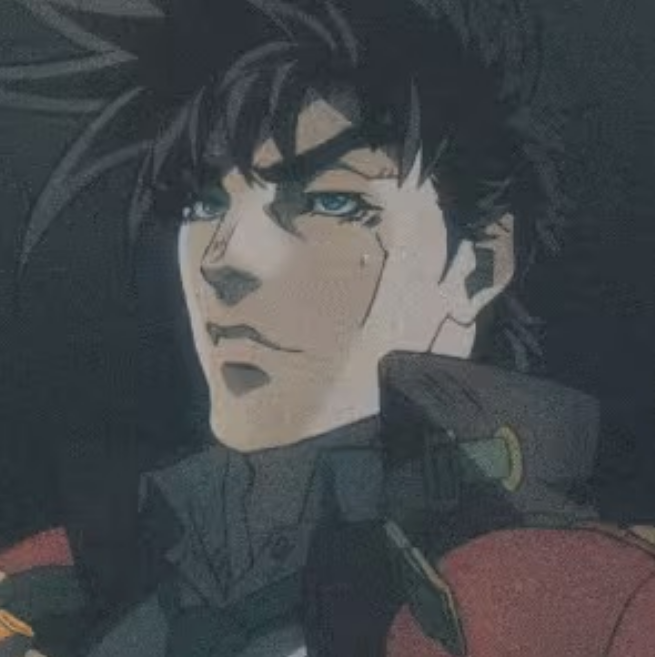
\includegraphics[width=0.06\linewidth]{p2.png}}
\renewcommand{\headrulewidth}{0.4pt}
\renewcommand{\footrulewidth}{0.4pt}

\begin{document}

\begin{center}
\Large\textbf{2012哈工大硕士考试试题：805物理光学}
\end{center}





\section*{一、填空题（20分）}
\begin{enumerate}
    \item \_\_\_\_\_称为波阵面。
    \item 球面波可以视为平面波的条件是\_\_\_\_\_。
    \item 产生干涉的条件是光波的\_\_\_\_\_。
    \item 光的相干性分为\_\_\_\_\_和\_\_\_\_\_。
    \item 法布里-波罗干涉仪的工作原理是\_\_\_\_\_，主要用途是\_\_\_\_\_。
    \item 光的偏振状态有\_\_\_\_\_。
    \item 观察屏距离衍射屏有限远的衍射称为\_\_\_\_\_，光源和观察屏距离衍射屏无穷远的衍射称为\_\_\_\_\_。
    \item 能够将自然光变为偏振光的器件称为\_\_\_\_\_。
\end{enumerate}
\section*{二、名词解释（27分）}
\begin{enumerate}
    \item 光波叠加的原理
    \item 光栅
    \item 艾里斑
    \item 双折射
    \item 条纹对比度
    \item 电光效应
    \item 巴比涅原理
    \item 补偿器
    \item 主截面
\end{enumerate}
\section*{三、选择题（18分）}
\begin{enumerate}
    \item 瑞利散射与拉曼散射的主要区别是\_\_\_\_\_\\(A)散射光与入射光强度关系\quad(B)散射光与入射光偏振度关系\quad (C)散射光与入射光相干性关系\quad (D)散射光与入射光波长关系
    \item 孔径相同的微波望远镜比光学望远镜分辨本领低的主要原因是\_\_\_\_\_。\\(A)星体发出的微波能量比可见光能量小\quad(B)微波更容易被大气吸收\quad(C)大气对微波的折射率小\quad(D)微波波长比可见光大
    \item 线偏振光入射光到一块方解石玻片上，其振动方向与主截面成$\theta$角，则波片的$o,e$光对应的出射光线振幅比值为\_\_\_\_\_。\\(A)$sin\theta$\quad(B)$cos\theta$(C)$tan\theta$\quad(D)$cot\theta$
    \item 在迈克尔逊干涉仪的一只光路中，垂直于光路放入折射率为$n$,厚度为$h$的透明介质片。放入后，两束光的光程差的改变量为\_\_\_\_\_。\\(A)$2(n-1)h$\quad (B)$2nh$\quad(C)$nh$\quad(D)$(n-1)h$
    \item 观察单缝弗朗和费衍射图样时，单缝宽度增加，屏上中央亮纹宽度\_\_\_\_\_。\\(A)不变\quad(B)变小\quad(C)变大\quad(D)无法确定
    \item （重复）假设某一介质对空气的临界角是60°，则光从空气射向此介质时的布儒斯特角是\_\_\_\_\_.\\(A)$tg^{-1}\sqrt({3}/2)$\qquad(B)$tg^{-1}(1/2)$\qquad(C)$tg^{-1}(2\sqrt{3}/3)$\qquad(D)$tg^{-1}2$
\end{enumerate}
\section*{四、简答题（30分）}
\begin{enumerate}
    \item 简述惠更斯-菲涅尔原理。
    \item 哪些因素决定光波的偏振态？
    \item 什么是相速度，群速度？何种情况下，群速度大于（小于）相速度？
    \item 简述全反射的发生的条件与特点。
    \item 一束光是否有可能包含两个正交的非相干态，但不是自然光？
    \item 简述可以使线偏振光旋转90度的方法。
\end{enumerate}
\section*{五、计算与分析（37分）}
\begin{enumerate}
    \item 一个线偏振光在玻璃中传播时的表达式为：$E=80co(\pi\times10^{15}\times (\frac{z}{0.7c}-t))$,求该光的频率，波长以及玻璃的折射率。
    \item 在正常情况下，人眼的瞳孔直径为$2.5mm$，人眼最敏感的波长为$550nm$。
          \begin{enumerate}
            \item 试求人眼的最小分辨角；
            \item 要分辨远处相距为$0.5m$的两光点，人眼至少离光点多近？
          \end{enumerate}
    \item 一束自然光正入射到重叠的两个偏振片上，分别计算：
          \begin{enumerate}
            \item 透射光强为入射光强的1/4事
            \item 透射光强为透射最大光强的3/4时，两个偏振片的夹角。
          \end{enumerate}
    \item 太阳光$600nm$，照在开孔$2cm$见方的暗室，开孔被一组宽度为$0.5d$的细丝覆盖，细丝的间距为$w$在孔后$d$处放置观察屏。以知太阳的角直径为$0.01rad$,分析下列情况观察屏上的现象。
          \begin{enumerate}
            \item $d=1mm,L=1mm$
            \item $d=1mm,L=10000mm$
            \item $d=0.005mm,L=-10000mm$
          \end{enumerate}       
          \begin{figure}[!htb]
                \centering
                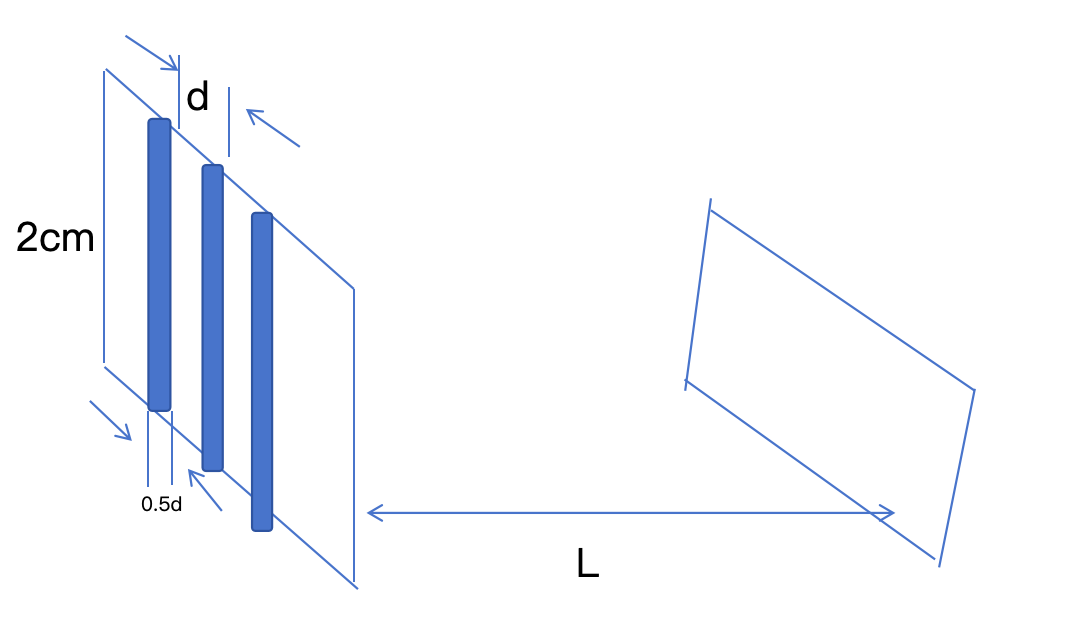
\includegraphics[width=0.7\linewidth]{121.png}
                \caption{下方标题}
          \end{figure}
\end{enumerate}
\section*{六、论述题（18分）}
\begin{enumerate}
    \item 某单位研制的光电设备光路简图如下图所示，系统调试后，在没有分光平板的情况下，成像系统A和系统B地像质均理想。加入分光板后，成像系统A的像质明显变差，而成像系统B像质理想。分析成像系统A存在像差可能的原因；并运用物理光学知识设计检测方案，验证分析结论。
         \begin{figure}[!htb]
                \centering
                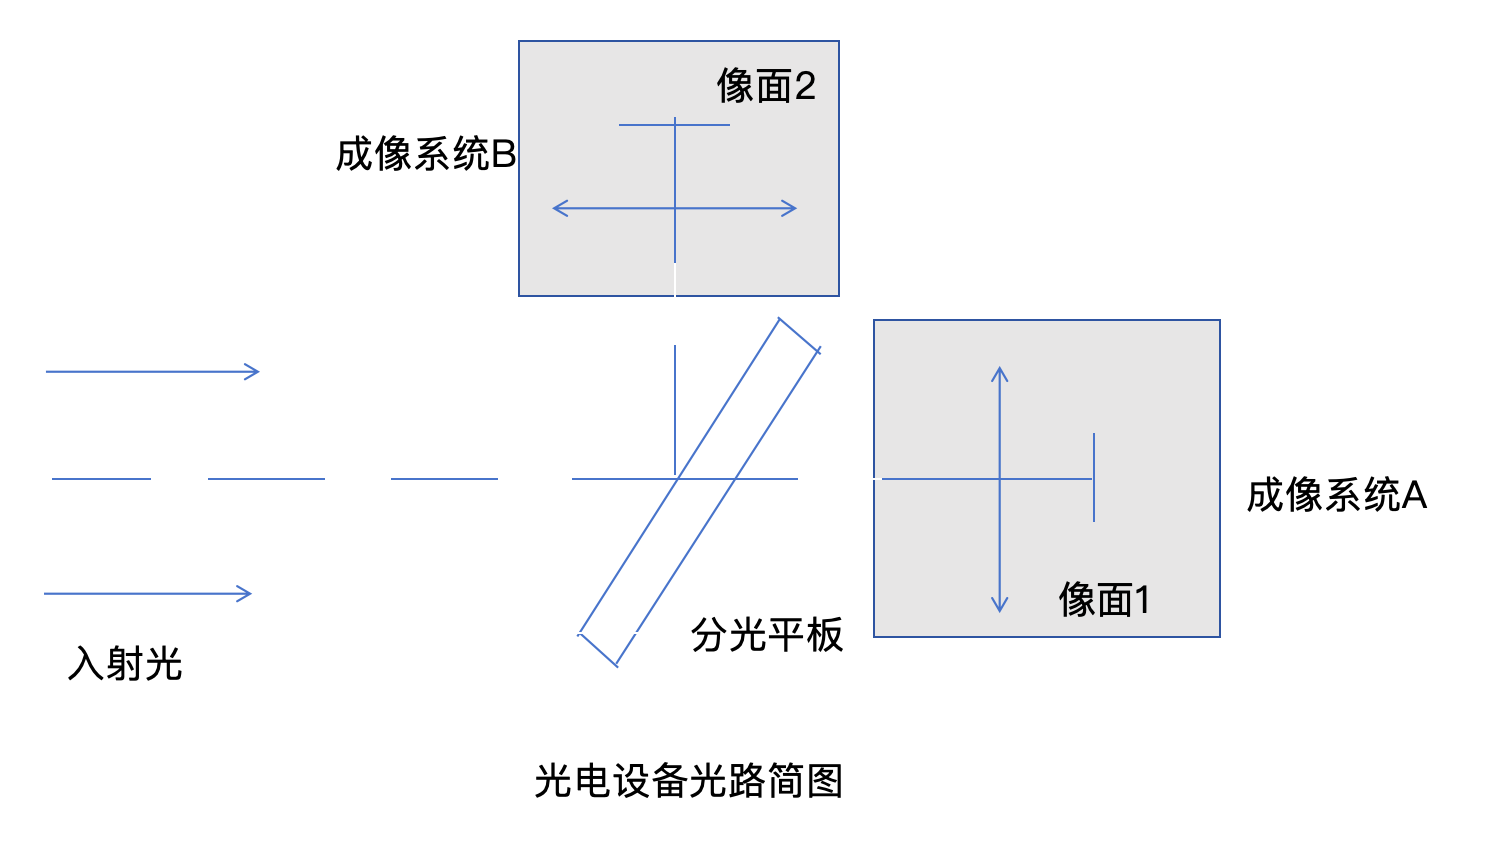
\includegraphics[width=0.7\linewidth]{122.png}
                
          \end{figure}
\end{enumerate}
\end{document}
